
\let\negmedspace\undefined
\let\negthickspace\undefined
\documentclass[journal]{IEEEtran}
\usepackage[a5paper, margin=10mm, onecolumn]{geometry}
%\usepackage{lmodern} % Ensure lmodern is loaded for pdflatex
\usepackage{tfrupee} % Include tfrupee package

\setlength{\headheight}{1cm} % Set the height of the header box
\setlength{\headsep}{0mm}     % Set the distance between the header box and the top of the text

\usepackage{gvv-book}
\usepackage{gvv}
\usepackage{cite}
\usepackage{amsmath,amssymb,amsfonts,amsthm}
\usepackage{algorithmic}
\usepackage{graphicx}
\usepackage{textcomp}
\usepackage{xcolor}
\usepackage{txfonts}
\usepackage{listings}
\usepackage{multicol}
\usepackage{enumitem}
\usepackage{mathtools}
\usepackage{gensymb}
\usepackage{comment}
\usepackage[breaklinks=true]{hyperref}
\usepackage{tkz-euclide} 
\usepackage{listings}
% \usepackage{gvv}                                        
\def\inputGnumericTable{}                                 
\usepackage{color}                                            
\usepackage{array}                                            
\usepackage{longtable}                                       
\usepackage{calc}                                             
\usepackage{multirow}                                         
\usepackage{hhline}                                           
\usepackage{ifthen}                                           
\usepackage{lscape}
\usepackage{tikz}
\usetikzlibrary{patterns}
\usepackage{amsmath}
\usepackage{tikz}
\usepackage[utf8]{inputenc}
\usepackage{pgfplots}
\pgfplotsset{compat=1.17}

\begin{document}
\bibliographystyle{IEEEtran}
\vspace{3cm}


\title{2015-CE-'1-13'}
\author{EE24BTECH11023}
%\maketitle
%\newpage
%\bigskip

{\let\newpage\relax\maketitle}

\renewcommand{\thefigure}{\theenumi}
\renewcommand{\thetable}{\theenumi}
\setlength{\intextsep}{10pt} % Space between text and floats


\numberwithin{equation}{enumi}
\numberwithin{figure}{enumi}
\renewcommand{\thetable}{\theenumi}
\begin{large}

\text{Q.1 to Q.5 carry 1 mark each \& Q.6 to Q.10 carry 2 marks each.}
\end{large}
\begin{enumerate}
    \item Extreme focus on syllabus and studying for tests has become such a dominant concern of Indian students that they close their minds to anything \underline{\hspace{1cm}} to the requirements of the exam.
    \begin{multicols}{4}
    \begin{enumerate}
        \item related
        \item extraneous
        \item outside
        \item useful
    \end{enumerate}
   \end{multicols}
    \item Select the pair that best expresses a relationship similar to that expressed in the pair:\\
    \textbf{Children:Pediatrician}.
     \begin{multicols}{2}
    \begin{enumerate}
        \item Adult: Orthopaedist
        \item Females: Gynaecologist
        \item Kidney: Nephrologist
        \item Skin: Dermatologist
    \end{enumerate}
      \end{multicols}
\item The Tamil version of \underline{\hspace{1cm}} John Abraham-starrer madras cafe \underline{\hspace{1cm}} cleared by the Censor Board with no cuts last week,but the film's distributors  \underline{\hspace{1cm}} no takers among the exhibitors for a release in Tamil Nadu \underline{\hspace{1cm}} this Friday.
 \begin{multicols}{2}
        \begin{enumerate}
        \item Mr.,was,found,on
        \item a,was,found,at
        \item the,was,found,on
        \item a,being,find at
        \end{enumerate}
      \end{multicols}
    \item If ROAD is written as URDG, then SWAN should be written as:
    \begin{enumerate}
        \item VXDQ
        \item VZDQ
        \item VZDP
        \item UXDQ
    \end{enumerate}
    \item A function $f(x)$ is linear and has a value of 29 at $x = -2$ and 39 at $x = 3$. Find its value at $x = 5$.
     \begin{multicols}{4}
    \begin{enumerate}
        \item 59
        \item 45
        \item 43
        \item 35
    \end{enumerate}
      \end{multicols}
    \item Alexander turned his attention towards India since he had conquered Persia. Which one of the statements below is logically valid and can be inferred from the above sentence?
    \begin{enumerate}
        \item Alexander would not have turned his attention towards India had he not conquered Persia.
        \item Alexander was not ready to rest on his laurels and wanted to march to India.
        \item Alexander was completely in control of his army and could command it to move towards India.
        \item Since Alexander’s kingdom extended to Indian borders after the conquest of Persia, he was keen to move further.
    \end{enumerate}
\item Most experts feel that in spite of possessing all the technical skills required to be a batsman of the highest order, he is unlikely to be so due to lack of requisite temperament. He was guilty of throwing away his wicket several times after working hard to lay a strong foundation. His critics pointed out that until he addressed this problem, success at the highest level will continue to elude him.\\
Which of the statement(s) below is/are logically valid and can be inferred from the above passage?
\begin{enumerate}
    \item[(i)] He was already a successful batsman at the highest level.
    \item[(ii)] He has to improve his temperament in order to become a great batsman.
    \item[(iii)] He failed to make many of his good starts count.
    \item[(iv)] Improving his technical skills will guarantee success.
\end{enumerate}
 \begin{multicols}{2}
\begin{enumerate}
\item (iii) and (iv) 
\item (ii) and (iii) 
\item (i), (ii) and (iii) 
\item (ii) only
\end{enumerate}
\end{multicols}
    \item The exports and imports (in crores of Rs) of a country from the year 2000 to 2007 are given in the following bar chart. In which year is the combined percentage increase in imports and exports the highest?
      \begin{figure}[H]
        \centering
        \begin{tikzpicture}
    \draw[thick] (-4,0) -- (4,0); 
    \draw[thick] (-4,1.5) -- (4,1.5);
    \draw[dashed] (-4,-0.5)--(-4,1.5);
    \draw[dashed](4,-0.5)--(4,1.5);
    \node at (0,1.8) {Laminar, fully-developed pipe flow};
    \draw[dashed] (-4.5,0.75) -- (4.5,0.75);
    \draw[->] (2,0.75) -- (3.5,0.75) node[above] {$u$};
    \draw[<->] (-0.75,0.75) -- (-0.75,1.5) node[midway, right] {$R$};
    \draw[->] (0.75,0.75) -- (0.75,1) node[midway, left] {$r$};
    \draw[|<->|] (-4,-0.3) -- (4,-0.3) node[midway, below] {$L$};
    \draw[->] (0.75,0.75) -- (1.25,0.75) node[midway, below] {$z$};
\end{tikzpicture}
  
    \end{figure}
    \item Choose the most appropriate equation for the function drawn as a thick line, in the plot below
      \begin{figure}[H]
        \centering
        \begin{tikzpicture}
\begin{axis}[
    ybar=5pt,
    bar width=12pt,
    width=10cm, height=7cm,
    ymin=0, ymax=350,
    ylabel={},
    symbolic x coords={Year 1, Year 2, Year 3},
    xtick=data,
    nodes near coords,
    legend style={at={(0.5,-0.15)},anchor=north,legend columns=-1},
    enlarge x limits=0.3,
    ymajorgrids=true,
    grid style=dashed
]
\addplot coordinates {(Year 1, 100) (Year 2, 200) (Year 3, 300)};
\addplot coordinates {(Year 1, 240) (Year 2, 296) (Year 3, 210)};
\legend{Number of units, Net Profit (*)}
\end{axis}
\end{tikzpicture}  
    \end{figure}
      \begin{enumerate}
        \item $x = y - |y|$
        \item $x = -(y - |y|)$
        \item $x = y + |y|$
        \item $x = -(y + |y|)$
    \end{enumerate}
 \item The head of a newly formed government desires to appoint five of the six selected members P,Q,R,S,T, and U to portfolios of home,Power,Defence,Telecom,and Finance.U does not want any portfolio if S gets one of the five.R wants either Home or Finance or no portfolio.Q says that if S gets either Power or Telecom,then she must get the other one.T insists on a portfolio if P gets one.\\
 Which is the valid distribution of portfolios?
    \begin{enumerate}
        \item P-Home, Q-Power, R-Defense, S-Telecom, T-Finance
        \item R-Home, S-Power, P-Defense, Q-Telecom, T-Finance
        \item P-Home, Q-Power, T-Defense, S-Telecom, U-Finance
        \item Q-Home, U-Power, T-Defense, R-Telecom, P-Finance
    \end{enumerate}
    
    \section*{Q.11 to Q.35 carry 1 mark each $\&$ Q.36 to Q.65 carry 2 marks each}
    \item For what value of $p$ will the following set of equations have no solution?
\[
    2x + 3y = 5
\]
\[
    3x + py = 10
\]
    \item The integral $\int_0^1 x \, dx$ with $x > 0$ is evaluated analytically as well as numerically using a single application of the trapezoidal rule. If $I$ is the exact value of the integral obtained analytically and $J$ is the approximate value obtained using the trapezoidal rule, which of the following statements is correct about their relationship?
    \begin{enumerate}
        \item $J > I$
        \item $J < I$
        \item $J = I$
        \item Insufficient data to determine the relationship
    \end{enumerate}
    \item Consider the following probability mass function (p.m.f) of a random variable X :
\[
    p(X) =
    \begin{cases}
        0, & \text{if } X = 0 \\
        1 - q, & \text{if } X = 1 \\
        q, & \text{otherwise}
    \end{cases}
    \]
    If $q = 0.4$, the variance of $X$ is \underline{\hspace{1cm}}.
\end{enumerate}
\end{document}